\documentclass[a4paper,10pt,french]{article}

\usepackage[utf8]{inputenc}
\usepackage[T1]{fontenc} 
\usepackage{graphicx,psfrag}
\usepackage[frenchb]{babel}
\usepackage{ae,aecompl}
\usepackage{float}
\usepackage{fancyhdr}
\renewcommand{\baselinestretch}{1.2}

%%%%%%%%%%%%%%%%%%%%%%%%%%%%%%%%%%%%%%%%%%%%%%%%%%%%%%%%%%%%

\setlength{\textwidth}{18cm}
\setlength{\textheight}{25cm}
\setlength{\oddsidemargin}{-1cm}
\setlength{\evensidemargin}{0cm}
\setlength{\topmargin}{-2cm}
\setlength{\parindent}{0cm}

%%%%%%%%%%%%%%%%%%%%%%%%%%%%%%%%%%%%%%%%%%%%%%%%%%%%%%%%%%%%
\pagestyle{fancy}

\renewcommand{\footrulewidth}{0.4 pt}
\renewcommand{\headrulewidth}{0 pt}

\newcommand{\fct}[1]{\texttt{#1}}
\newcommand{\menu}[1]{\texttt{#1}}
\newcommand{\code}[1]{\texttt{#1}}
\newcommand{\pkg}[1]{\textsf{#1}}

%%%%%%%%%%%%%%%%%%%%%%%%%%%%%%%%%%%%%%%%%%%%%%%%%%%%%%%%%%%%

\begin{document}
\thispagestyle{empty}

%\vspace*{-3cm}~\\
\hspace*{-0.5cm}

%%%%%%%%%%%%%%%%%%%%%%%%%%%% Titre %%%%%%%%%%%%%%%%%%%%%%%%%%%%%%%%%%%%
\begin{center}
\LARGE Statistiques descriptives avec \textsf{R}
\end{center}
\bigskip

%%%%%%%%%%%%%%%%%%%%%%%%%%%%%%%%%%%%%%%%%%%%%%%%%%%%%%%%%%%%%%%%%%%%%%
\section{Statistiques descriptives: représentation de variables}
\subsection{Représenter une variable qualitative}
Nous allons rentrer des données \og à la main\fg{} pour une variable
qualitative. Cette variable représente l'appartenance à un groupe
(parmi 3 groupes) et prend 3 modalités \texttt{g1}, \texttt{g2} et
\texttt{g3}. Les 2 premiers individus sont dans le groupe 1, les 3 suivants dans le groupe 2  et le dernier dans le groupe 3:
\begin{verbatim}
ybrut <- c("g1","g1","g2","g2","g2","g3")
print(ybrut)
summary(ybrut)
\end{verbatim}
Que fait le dernier ordre ci-dessus ?  Nous devons
transformer ce vecteur (de caractères) en variable qualitative (nommée
\texttt{factor} sous \textsf{R}):
\begin{verbatim}
y <- factor(ybrut)
\end{verbatim}
Que font les ordres suivants ?
\begin{verbatim}
levels(y)
nlevels(y)
table(y)
sum(table(y))
table(y)/sum(table(y))*100
\end{verbatim}
Tracer les effectifs de chaque modalité dans un diagramme en barre:
\begin{verbatim}
barplot(table(y))
\end{verbatim}
Tracer les pourcentages de chaque modalité dans un diagramme en barre:
\begin{verbatim}
barplot(table(y)/sum(table(y))*100,ylab="pourcentages",xlab="groupes")
\end{verbatim}
Que font les options \texttt{xlab} et \texttt{ylab} ?

Copier le dernier graphique dans un document word ou openoffice.

Que fait le résumé numérique d'une variable qualitative ?
\begin{verbatim}
summary(y)
\end{verbatim}

\subsection{Représenter une variable quantitative continue}
Représentons une variable quantitative continue. Ouvrir le fichier
\texttt{varquant.r} et exécuter son contenu (couper coller son contenu
ou utiliser l'icône de tinn-R).


Que fait le résumé numérique d'une variable quantitative (continue) ?
\begin{verbatim}
summary(y)
\end{verbatim}
Trouver sur les deux graphiques ci-dessous la différence et expliquez la.
\begin{verbatim}
hist(y,freq=TRUE)
hist(y,freq=FALSE)
\end{verbatim}

Que font toutes les options pour ce graphique
\begin{verbatim}
hist(y,freq=FALSE,breaks=10,xlab="huile",main="Histogramme")
\end{verbatim}
Que fait cette option
\begin{verbatim}
hist(y,freq=FALSE,breaks=c(15,18,25,30,36))
\end{verbatim}
Expliquer tous les ordres ci-dessous
\begin{verbatim}
boxplot(y,xlab="",ylab="teneur en huile")
mean(y)
abline(h=mean(y))
quantile(y)
median(y)
abline(h=median(y),col=2)
\end{verbatim}
Conclusion: l'histogramme est tracé grae à \texttt{hist} avec l'option
\texttt{freq=FALSE}.

Un autre estimateur de la densité (estimateur à noyau) est disponible afin d'estimer la densité par une fonction continue
\begin{verbatim}
density(x, ...)
\end{verbatim}
Retourne les coordonnées x et y d'un \emph{estimateur} de la densité du vecteur de données \code{x}. L'argument \code{bw} indique la largeur de fenetre (plus elle est grande plus la courbe est lisse)
\begin{verbatim}
> normal=rnorm(100)
> ndens=density(normal, width=1.2)
> hist(normal, probability=T)
> lines(ndens)
\end{verbatim}
 
\subsection{Représenter une variable quantitative discrète}
Représentons une variable quantitative discrète: le nombre d'enfant
par famille. Nous allons rentrer des données \og à la main\fg{} les
valeurs de cette variable. La première famille possède 5 enfants, la
second n'en a pas, la troisième en possède 2 enfants, la quatrième 2 et la cinquième n'en a pas.
\begin{verbatim}
y <- c(5,0,2,2,0)
\end{verbatim}

Que font les commandes suivantes
\begin{verbatim}
unique(y)
sort(unique(y))
table(y)
\end{verbatim}
Le diagramme en barre des effectifs est le diagramme suivant
\begin{verbatim}
plot(sort(unique(y)),table(y),type="h",ylim=c(0,max(table(y))))
\end{verbatim}

En général, dès que les valeurs possibles sont assez nombreuses (par
exemple 7 ou 10 ou plus) la variable quantitative discrète est
assimilée à une variable quantitative continue.  La distinction
quantitatif discret ou continue n'existe pas sous \textsf{R}, les deux sont des variables numériques (\texttt{numeric}).

\subsection{Données des tournesols}
\begin{enumerate}
\item Importer le tableau \texttt{tournesol.csv} qui contient les variables décrites dans le tableau \ref{tab:variables:plantes}.  Ce tableau sera affecté dans un objet appelé \texttt{tpropre}.
\begin{table}[H]
  \centering
  \begin{tabular}{cl}\hline\hline
Code variable& Descriptif variable\\\hline
    ecotype & code plante \\
plt & numéro du plant d'un écotype donné\\
etat & état d'origine de la plante (aux USA)\\
longitude& longitude du lieu de collecte (aux USA)\\
latitude& latitude du lieu de collecte (aux USA)\\
haut& hauteur des plants\\
semflo& jour de floraison (écart en jour par rapport au premier mai)\\
rambas&note de ramification basale (entre 0 aucune et 4 maximum)\\
longfeu&longueur du cumulée du limbe et du pétiole (cm ?)\\ 
grlon&longueur maxi de la graine (mm, moyenne sur 15 graines minimum)\\
huile&pourcentage d'huile\\\hline
  \end{tabular}
  \caption{Variables mesurées sur les tournesols (dans la station d'essai aux environs de Montpellier).}
  \label{tab:variables:plantes}
\end{table}
\item Donner pour chaque variable son type (variable qualitative,
  quantitative discrète, quantitative continue).
\item Effectuer un résumé numérique du tableau de données \texttt{tpropre}:
\begin{verbatim}
summary(tpropre)
\end{verbatim}
\item Quelles sont les variables qui sont reconnues comme variables quantitatives et comme variables qualitatives ?
\item Donner à chaque variable le type voulu grâce à \texttt{factor} ou \texttt{as.numeric}
\end{enumerate}



\subsection{Deux variables quantitatives continues}
Par defaut \textsf{R} trace des points (\texttt{type="p"}) aux
coordonnées fournies (ci-dessous l'ordonnée est la variable
\texttt{huile} et l'abscisse la variable \texttt{grlon}). Détailler le
rôle des options
\begin{verbatim}
plot(huile~grlon,data=tpropre)
plot(huile~grlon,data=tpropre,pch="+")
plot(huile~grlon,data=tpropre,col=2,pch="+")
\end{verbatim}

Traçons des lignes
\begin{verbatim}
plot(huile~grlon,data=tpropre,type="l")
\end{verbatim}
Qu'a t-on fait ?

\subsection{Deux variables qualitatives: tableau de contingence}
Utilisez l'ordre suivant
\begin{verbatim}
table(tpropre[,"ecotype"],tpropre[,"etat"])
\end{verbatim}
Que renvoit il ?

\subsection{Données des tournesols (suite)}
\begin{enumerate}
\item Calculer la moyenne empirique des variables \texttt{huile, grlon} et \texttt{longfeu}.
\item Pour ces mêmes variables donner leurs quartiles empiriques.
\item Pour ces mêmes variables les représenter par un boxplot.
\item Pour ces mêmes variables calculer leur variance empirique.
\item Représenter graphiquement chacune des variables et exporter ces
  représentations graphiques dans un document word ou openoffice.
\end{enumerate}
\section{Manipuler des données}
\subsection{Importation (exercice)}
Importer les tableaux \code{test1.csv},
\code{test2.csv} et \code{test3.csv} dans les variables \code{don1}, \code{don2}, \code{don3}.
\subsection{Fusionner des tableaux}
Exécuter et commenter:
\begin{verbatim}
> toto.1 <- cbind(don1,don3)
> toto.1
> montab = rbind(don1,don2)
> montab
> rbind(don1,don3)
> objects()
> rm(toto.1,montab)
> objects()
\end{verbatim}
\subsection{Fusionner des tableaux}
Il est possible de fusionner deux tableaux selon une clef (cf. fusion
de 2 tables dans les bases de données), grâce à l'ordre classique
\texttt{merge}

\begin{figure}[H]
  \centering
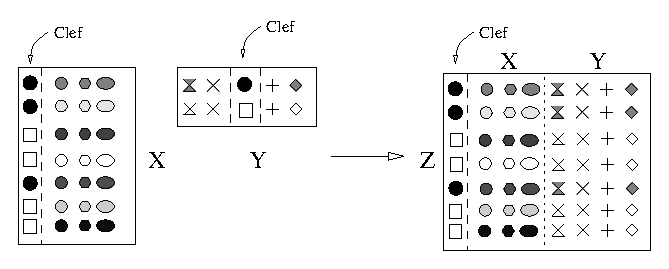
\includegraphics[width=\textwidth]{bind}
  \caption{Fusion par clef: \texttt{merge(X,Y,by="clef")} où \texttt{clef} est le nom d'une variable commune à \texttt{X} et \texttt{Y}.}
  \label{fig:merge}
\end{figure}
Importer les données du fichier \texttt{tournesol\string_propre.csv}
(dans que l'on nommera \texttt{tpropre}) ainsi que celle du fichier 
\texttt{meteo\string_tournesol.csv} (dans un tableau nommé \texttt{meteo}\label{sec:importation}).
Faire fusionner les tableaux \texttt{tpropre} et \texttt{meteo}
grâce à la clef \texttt{ecotype}.
\section{Facteurs et fonctions}
\begin{enumerate}

\item Réimporter éventuellement l'objet \code{mtcars} grâce à \code{data(mtcars)}.
\item Donner un résumé numérique de chaque variable de la matrice
  \texttt{mtcars} (voir \texttt{summary})\label{item:1}. 
\item Créer un facteur (de nom \texttt{conso}) en découpant en classe
  la variable \texttt{mpg} (de la matrice \texttt{mtcars}). Le découpage sera fait de 5 en 5 en partant de 10 (voir \texttt{cut, seq}). 
\item Afficher les niveaux (ou modalités) de \texttt{conso} (\texttt{levels}). 
\item Créer \texttt{conso2} égal à \texttt{conso}.
\item Fusionner la premiere et la seconde modalité de  \texttt{conso2} en une seule de nom \texttt{"fuse"} (\texttt{levels}).
\item Transformer \texttt{conso} en facteur ordonné (\texttt{ordered}). 
\item Voir les effectif de chaque modalité (\texttt{table})
\item Voir les pourcentages de chaque modalité (\texttt{table, length})
\item Faire un résumé numérique de \texttt{conso} et voir la différence 
avec une variable numérique (question \ref{item:1}). 
\item Faire une moyenne de chaque variable de la matrice \texttt{mtcars} (\texttt{apply} ET \texttt{colMeans}). 
\item Faire une somme de chaque variable de la matrice \texttt{mtcars} (\texttt{apply} et  ET \texttt{colSums} ET par une boucle)). 
\item Calculer la médiane somme de chaque variable de la matrice \texttt{mtcars} (\texttt{apply})). 
\item Créer une fonction pour calculer $n!=1\times 2\times \ldots (n-1)\times n$
\begin{itemize}
\item par une boucle \texttt{for},
\item par une boucle \texttt{while},
\item sans boucle (\texttt{prod}),
\item par une fonction mathématique intégrée. 
\end{itemize}
\item Créer une fonction pour les écarts absolus à la moyenne d'un
  vecteur \texttt{x} ($MAD=\frac{1}{n}\sum_{i=1}^n{}{|x_i-\bar x|}$ où $\bar
  x=\frac{1}{n}\sum_{i=1}^{n}{x_i}$. 
\item utiliser cette fonction pour calculer l'écart à la moyenne (MAD) pour chaque colonne de la matrice \texttt{mtcars} (\texttt{apply}). 
\item Calculer la moyenne, pour chaque niveau de \texttt{conso}, de toutes les colonnes de la matrice \texttt{mtcars} (\texttt{apply})) sauf la première ie. 
\item Calculer la moyenne par niveau de \texttt{conso} de toutes les colonnes de la matrice \texttt{mtcars} sauf la première (ipour les 10 colonnes de mtcars il faut 5 moyennes, une par niveau de \texttt{conso}) ; voir \texttt{aggregate}. 
\end{enumerate}

\end{document}
%%% Local Variables: 
%%% mode: latex
%%% TeX-master: t
%%% End: 
